\documentclass[openany]{book}

\usepackage[margin=1in]{geometry}
\usepackage{amsmath,amsfonts,amsthm, amssymb}
\usepackage{yhmath}
\usepackage{mathrsfs}
\usepackage{mathtools}
\usepackage{xcolor}
\usepackage{graphicx}
\usepackage{comment}
\usepackage{tikz-cd}
\usepackage{quiver}
\renewcommand{\familydefault}{ppl}
\newcommand{\tr}{\text{tr}}
\newcommand{\R}{\mathbb{R}}
\newcommand{\E}{\mathbb{E}}
\newcommand{\Z}{\mathbb{Z}}
\newcommand{\C}{\mathbb{C}}
\newcommand{\F}{\mathbb{F}}
\newcommand{\la}{\langle}
\newcommand{\ra}{\rangle}
\newcommand{\colim}{\text{colim}}
\DeclareMathOperator{\im}{im}
\let\oldemptyset\emptyset
\let\emptyset\varnothing
\newcommand{\tor}{\text{Tor}}
\newcommand{\id}{\text{id}}
\newcommand{\ext}{\text{Ext}}
\newcommand{\ptop}{\text{PTop}}
\newcommand{\pt}{\text{pt}}
\newcommand{\ach}{\text{Ach}}
\newcommand{\Q}{\mathbb{Q}}
\newcommand{\gal}{\text{Gal}}


\usepackage{thmtools,thm-restate}

% Fixing mdframed skip below
% See https://tex.stackexchange.com/a/292090/143086
\usepackage[framemethod=TikZ]{mdframed}
\usepackage{xpatch}
\makeatletter
\xpatchcmd{\endmdframed}
	{\aftergroup\endmdf@trivlist\color@endgroup}
	{\endmdf@trivlist\color@endgroup\@doendpe}
	{}{}
\makeatother

\definecolor{huilightpink}{HTML}{fff2fe}
\definecolor{huidarkpink}{HTML}{d955b7}
\declaretheoremstyle[
	mdframed={
		backgroundcolor=huilightpink,
		linecolor=huidarkpink,
		rightline=false,
		topline=false,
		bottomline=false,
		linewidth=2pt,
		innertopmargin=5pt,
		innerbottommargin=8pt,
		innerleftmargin=8pt,
		leftmargin=-2pt,
		skipbelow=2pt,
		nobreak
	},
	headfont=\normalfont\bfseries\color{huidarkpink}
]{huipinkbox}
\declaretheorem[style=huipinkbox,name=Theorem,within=chapter]{thm}
\declaretheorem[style=huipinkbox,name=Theorem,sibling=thm]{theorem}




\begin{comment}
\definecolor{huilightyellow}{HTML}{fff5d6}
\definecolor{huidarkyellow}{HTML}{fcad03}
\declaretheoremstyle[
	mdframed={
		backgroundcolor=huilightyellow,
		linecolor=huidarkyellow,
		rightline=false,
		topline=false,
		bottomline=false,
		linewidth=2pt,
		innertopmargin=5pt,
		innerbottommargin=8pt,
		innerleftmargin=8pt,
		leftmargin=-2pt,
		skipbelow=2pt,
		nobreak
	},
	headfont=\normalfont\bfseries\color{huidarkyellow}
]{huiyellowbox}
\declaretheorem[style=huiyellowbox,name=Proposition,within=chapter]{prop}
\end{comment}



\definecolor{huilightpurple}{HTML}{faf2ff}
\definecolor{huidarkpurple}{HTML}{912ed9}
\declaretheoremstyle[
	mdframed={
		backgroundcolor=huilightpurple,
		linecolor=huidarkpurple,
		rightline=false,
		topline=false,
		bottomline=false,
		linewidth=2pt,
		innertopmargin=5pt,
		innerbottommargin=8pt,
		innerleftmargin=8pt,
		leftmargin=-2pt,
		skipbelow=2pt,
		nobreak
	},
	headfont=\normalfont\bfseries\color{huidarkpurple}
]{huipurplebox}
\declaretheorem[style=huipurplebox,name=Proposition,within=chapter]{prop}



% \definecolor{huilightpurple}{HTML}{faf2ff}
% \definecolor{huidarkpurple}{HTML}{912ed9}
% \declaretheoremstyle[
% 	mdframed={
% 		backgroundcolor=huilightpurple,
% 		linecolor=huidarkpurple,
% 		rightline=false,
% 		topline=false,
% 		bottomline=false,
% 		linewidth=2pt,
% 		innertopmargin=5pt,
% 		innerbottommargin=8pt,
% 		innerleftmargin=8pt,
% 		leftmargin=-2pt,
% 		skipbelow=2pt,
% 		nobreak
% 	},
% 	headfont=\normalfont\bfseries\color{huidarkpurple}
% ]{huipurplebox}
\declaretheorem[style=huipurplebox,name=Lemma,within=chapter]{lem}


\definecolor{lightpink}{HTML}{f0f6fc}
\definecolor{darkpink}{HTML}{2c72b8}
\declaretheoremstyle[
	mdframed={
		backgroundcolor=lightpink,
		linecolor=darkpink,
		rightline=false,
		topline=false,
		bottomline=false,
		linewidth=2pt,
		innertopmargin=5pt,
		innerbottommargin=8pt,
		innerleftmargin=8pt,
		leftmargin=-2pt,
		skipbelow=2pt,
		nobreak
	},
	headfont=\normalfont\bfseries\color{darkpink}
]{pinkbox}
\declaretheorem[style=pinkbox,name=Definition,within=chapter]{defn}


\definecolor{huilightblue}{HTML}{edf9ff}
\definecolor{huidarkblue}{HTML}{4b79db}
\declaretheoremstyle[
	mdframed={
		backgroundcolor=huilightblue,
		linecolor=huidarkblue,
		rightline=false,
		topline=false,
		bottomline=false,
		linewidth=2pt,
		innertopmargin=5pt,
		innerbottommargin=8pt,
		innerleftmargin=8pt,
		leftmargin=-2pt,
		skipbelow=2pt,
		nobreak
	},
	headfont=\normalfont\bfseries\color{huidarkblue}
]{huiblueblox}
\declaretheorem[style=huiblueblox,name=Example,within=chapter]{example}



% \definecolor{huilightblue}{HTML}{edf9ff}
% \definecolor{huidarkblue}{HTML}{4b79db}
% \declaretheoremstyle[
% 	mdframed={
% 		backgroundcolor=huilightblue,
% 		linecolor=huidarkblue,
% 		rightline=false,
% 		topline=false,
% 		bottomline=false,
% 		linewidth=2pt,
% 		innertopmargin=5pt,
% 		innerbottommargin=8pt,
% 		innerleftmargin=8pt,
% 		leftmargin=-2pt,
% 		skipbelow=2pt,
% 		nobreak
% 	},
% 	headfont=\normalfont\bfseries\color{huidarkblue}
% ]{huiblueblox}
% \declaretheorem[style=huiblueblox,name=Example,within=chapter]{example}

% \declaretheoremstyle[
% 	mdframed={
% 		backgroundcolor=huilightblue,
% 		linecolor=huidarkblue,
% 		rightline=false,
% 		topline=false,
% 		bottomline=false,
% 		linewidth=2pt,
% 		innertopmargin=5pt,
% 		innerbottommargin=8pt,
% 		innerleftmargin=8pt,
% 		leftmargin=-2pt,
% 		skipbelow=2pt,
% 		nobreak
% 	},
% 	headfont=\normalfont\bfseries\color{huidarkblue}
% ]{huiblueblox}
\declaretheorem[style=huiblueblox,name=Problem,within=chapter]{prob}



% \declaretheoremstyle[
% 	mdframed={
% 		backgroundcolor=huilightblue,
% 		linecolor=huidarkblue,
% 		rightline=false,
% 		topline=false,
% 		bottomline=false,
% 		linewidth=2pt,
% 		innertopmargin=5pt,
% 		innerbottommargin=8pt,
% 		innerleftmargin=8pt,
% 		leftmargin=-2pt,
% 		skipbelow=2pt,
% 		nobreak
% 	},
% 	headfont=\normalfont\bfseries\color{huidarkblue}
% ]{huiblueblox}
\declaretheorem[style=huiblueblox,name=Exercise,within=chapter]{exer}
\declaretheorem[style=huipinkbox, name=Corollary, within=chapter]{cor}





















\newcommand{\nirwarnsymbol}{%
	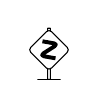
\begin{tikzpicture}[baseline=(x.base)]
		\draw[rounded corners=.01em] (-.05em,-1.07em)rectangle(.05em,.78em);
		\draw[fill=white,rounded corners=1.3] (0,.75em)--(.75em,0)--(0,-.75em)--(-.75em,0)--cycle;
		\draw[line width=0.2mm, line cap=round](-.4em,-1.07em)--(.4em,-1.07em);
		\node(x) at (0,0em) {};
		% Thank you https://tex.stackexchange.com/a/262510
		\draw[
			line cap=but,
			line join=round,
			x=.5em,
			line width=0.5mm,
			y=1*(height("Z")-\pgflinewidth)*(1-sin(10)),
			rotate=-10,
			rounded corners=1.5pt,
		](-0.57, 0.57) -- (0.57, 0.57) -- (-0.57, -0.57) -- (0.57, -0.57);
	\end{tikzpicture}%
}

%%%%%%%%%%%%%%%%%%%%%%%%%%%%%%%%%%%%%%%%%%%% MARGINS
\usepackage{marginnote}
% Thank you https://tex.stackexchange.com/a/472882
% Makes marginnotes always appear on the left, apparently
%
\makeatletter
\long\def\@mn@@@marginnote[#1]#2[#3]{%
	\begingroup
		\ifmmode\mn@strut\let\@tempa\mn@vadjust\else
			\if@inlabel\leavevmode\fi
			\ifhmode\mn@strut\let\@tempa\mn@vadjust\else\let\@tempa\mn@vlap\fi
		\fi
		\@tempa{%
			\vbox to\z@{%
				\vss
				\@mn@margintest
				\if@reversemargin\if@tempswa
						\@tempswafalse
					\else
						\@tempswatrue
				\fi\fi

					\llap{%
						\vbox to\z@{\kern\marginnotevadjust\kern #3
							\vbox to\z@{%
								\hsize\marginparwidth
								\linewidth\hsize
								\kern-\parskip
								%\mn@parboxrestore
								\marginfont\raggedleftmarginnote\strut\hspace{\z@}%
								\ignorespaces#1\endgraf
								\vss
							}%
							\vss
						}%
						\if@mn@verbose
							\PackageInfo{marginnote}{xpos seems to be \@mn@currxpos}%
						\fi
						\begingroup
							\ifx\@mn@currxpos\relax\else\ifx\@mn@currpos\@empty\else
									\kern\@mn@currxpos
							\fi\fi
							\ifx\@mn@currpage\relax
								\let\@mn@currpage\@ne
							\fi
							\if@twoside\ifodd\@mn@currpage\relax
									\kern-\oddsidemargin
								\else
									\kern-\evensidemargin
								\fi
							\else
								\kern-\oddsidemargin
							\fi
							\kern-1in
						\endgroup
						\kern\marginparsep
					}%
			}%
		}%
	\endgroup
}
\makeatother
%
% Mostly for todonotes
\renewcommand{\marginpar}{\marginnote}
%%%%%%%%%%%%%%%%%%%%%%%%%%%%%%%%%%%%%%%%%%%% /MARGINS

\definecolor{nirlightred}{RGB}{250, 220, 220}
\definecolor{nirdarkred}{HTML}{f40000}
\declaretheoremstyle[
	mdframed={
		backgroundcolor=nirlightred,
		linecolor=nirdarkred,
		rightline=false,
		topline=false,
		bottomline=false,
		linewidth=2pt,
		innertopmargin=5pt,
		innerbottommargin=8pt,
		innerleftmargin=8pt,
		leftmargin=-2pt,
		skipbelow=2pt,
		nobreak
	},
	headfont=\normalfont\bfseries\color{nirdarkred}
]{nirredbox}

% \makeatletter
% \declaretheorem[
% 	style=nirredbox,
% 	name=Warning,
% 	sibling=thm,
% 	% without \leavevmode, the first item in a list gets misformatted
% 	postheadhook={\leavevmode\marginnote{\nirwarnsymbol}[-3pt]%
% 	\ifthmt@thisistheone% restatable makes alignment weird
% 		\hspace{-2.2pt}%
% 	\fi}
% ]{warn}
% \makeatother

\newcommand{\nirideasymbol}{%
	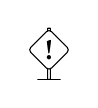
\begin{tikzpicture}[baseline=(x.base)]
		\draw[rounded corners=.01em] (-.05em,-1.07em)rectangle(.05em,.78em);
		\draw[fill=white,rounded corners=1.3] (0,.75em)--(.75em,0)--(0,-.75em)--(-.75em,0)--cycle;
		\draw[line width=0.2mm, line cap=round](-.4em,-1.07em)--(.4em,-1.07em);
		\node(x) at (0,0em) {};
		\node at (0,0em) {{\textbf{!}}};
	\end{tikzpicture}%
}
\renewcommand{\nirwarnsymbol}{%
	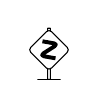
\begin{tikzpicture}[baseline=(x.base)]
		\draw[rounded corners=.01em] (-.05em,-1.07em)rectangle(.05em,.78em);
		\draw[fill=white,rounded corners=1.3] (0,.75em)--(.75em,0)--(0,-.75em)--(-.75em,0)--cycle;
		\draw[line width=0.2mm, line cap=round](-.4em,-1.07em)--(.4em,-1.07em);
		\node(x) at (0,0em) {};
		% Thank you https://tex.stackexchange.com/a/262510
		\draw[
			line cap=but,
			line join=round,
			x=.5em,
			line width=0.5mm,
			y=1*(height("Z")-\pgflinewidth)*(1-sin(10)),
			rotate=-10,
			rounded corners=1.5pt,
		](-0.57, 0.57) -- (0.57, 0.57) -- (-0.57, -0.57) -- (0.57, -0.57);
	\end{tikzpicture}%
}
\makeatletter
\declaretheorem[
	style=nirredbox,
	name=Idea,
	sibling=thm,
	% without \leavevmode, the first item in a list gets misformatted
	postheadhook={\leavevmode\marginnote{\nirideasymbol}[-3pt]%
	\ifthmt@thisistheone% restatable makes alignment weird
		\hspace{-2.2pt}%
	\fi}
]{idea}

\declaretheorem[
	style=nirredbox,
	name=Warning,
	sibling=thm,
	% without \leavevmode, the first item in a list gets misformatted
	postheadhook={\leavevmode\marginnote{\nirwarnsymbol}[-3pt]%
	\ifthmt@thisistheone% restatable makes alignment weird
		\hspace{-2.2pt}%
	\fi}
]{warn}
\makeatother

\title{Calc III Sections
\\ 
\vspace{0.4cm}
\large Fall 2025}




\date{\today}
\author{Hui Sun}


\begin{document}

\maketitle

% \tableofcontents
\newpage


\begin{center}
    \Large Calc III-Week 5 (9/22-9/26)
\end{center}

\renewcommand\thesection{\arabic{section}}

\noindent
Topics: (1) properties of derivatives, (2) directional derivatives, (3) gradient.


% (Section 2.5 on the multivariable chain rule and Section 2.6 on gradients and directional derivatives.

% I would like you to spend about 15-20 minutes going through some chain rule problems e.g. something like problems 7 or 8 from Section 2.5. One problem I really like that reviews multiple different concepts is 11 from Section 2.5 If you could present this problem, I think that would be good for the students
 
% key concept: the matrix of partial derivatives. 
 
% Please use the rest of the time to start discussing Section 2.6, specifically focusing on pg. 135-139. I will try to go through these pages on Monday, but I may have to go quickly. Reviewing all this material with simple examples is what I would recommend. Some problems that could be relevant are 3, 6, and 7 from Section 2.6).


\begin{defn}[path]
    A \textbf{path} $c$ is a map $c: [a,b]\to \R^n$. We can write $c(t)=(c_1(t), \dots, c_n(t))$. If $c$ is differentiable, then we can define the \textbf{velocity} of $c$ at any $t_0\in [a,b]$ as 
    \begin{equation*}
        c'(t_0)=\left(c_1'(t_0), \dots, c_n'(t_0)\right)
    \end{equation*}
    The velocity vector of $c$ at $t_0$ is also a \textbf{tangent} vector to $c$ at $t_0$. The \textbf{speed} of the path $c$ at $t_0$ is the length of the velocity vector $\|c'(t_0)\|$.
\end{defn}

\begin{defn}[tangent line to a path]
    Let $c:[a,b]\to\R^n$ be a path, if $c'(t_0)\neq 0$, then the \textbf{tangent line} at $x_0$ is given by 
    \begin{equation*}
        l(t)=c(t_0)+c'(t_0)(t-t_0)
    \end{equation*}
\end{defn}





\begin{prop}
    Let $f:U\subset\R^n\to\R^m$ be differentiable at $x_0$, then the derivative of $f$ at $x_0$ is an $m\times n$ matrix $Df(x_0)=\left(\frac{\partial f_i}{\partial x_j}\right)_{ij}$. The derivative follows the same properties as derivative for single variable functions:
    \begin{enumerate}
        \item Let $c\in\R$, then 
        \begin{equation*}
            D(cf)(x_0)=cDf(x_0) \tag {multiplication of a matrix by constant $c$}
        \end{equation*}
        \item Let $g: U\subset\R^n\to\R^m$ also be differentiable at $x_0$, then 
        \begin{equation*}
            D(f+g)(x_0)=Df(x_0)+Dg(x_0) \tag{sum of two matrices}
        \end{equation*}
        \item Let $h_1: U\subset\R^n\to\R, h_2: U\subset\R^n\to\R$,then 
        \begin{equation*}
            D(h_1h_2)(x_0)=Dh_1(x_0)h_2(x_0)+h_1(x_0)Dh_2(x_0) \tag{product rule}
        \end{equation*}
        and if $h_2\neq 0$ on $U$.
        \begin{equation*}
            D(h_1/h_2)(x_0)=\frac{Dh_1(x_0)h_2(x_0)-h_1(x_0)Dh_2(x_0)}{h_2^2(x_0)} \tag{quotient rule}
        \end{equation*}
        \item Let $g: U\subset\R^n\to\R^m, f:V\subset\R^m\to\R^p$ such that $g(U)\subset V$, then 
        \begin{equation*}
            D(f\circ g)(x_0)=Df(g(x_0))Dg(x_0) \tag{chain rule}
        \end{equation*}
    \end{enumerate}
\end{prop}

\begin{defn}[directiona derivative]
    Let $f:\R^3\to\R$, be differentiable, then the directional directive at $x_0\in\R^3$ in the direction of a \textbf{unit vector} $v$ is given by 
    \begin{equation*}
        \nabla f(x_0)\cdot v=\left[\frac{\partial f}{\partial x_1}(x_0)\right]v_1+\left[\frac{\partial f}{\partial x_2}(x_0)\right]v_2+\left[\frac{\partial f}{\partial x_3}(x_0)\right]v_3
    \end{equation*}
    where $v=(v_1,v_2,v_3)$.
\end{defn}

\begin{prop}
    Suppose that $\nabla f(x_0)\neq 0$, then the direction for which $f$ increases the fastest at $x_0$ is along $\nabla f(x_0)$.
\end{prop}


\begin{prop}
    Let $f:\R^3\to\R$ be differentiable, let $S$ be a level surface of $f$, i.e., $S$ is a surface described by 
    \begin{equation*}
        f(x,y,z)=k
    \end{equation*}
    were $k$ is some constant. Let $(x_0,y_0,z_0)\in S$, then
    \begin{equation*}
        \nabla f(x_0,y_0,z_0) \text{ is normal to the level surface at } (x_0,y_0,z_0)
    \end{equation*}
    This means if $c(t)$ is a path in $S$, and $v(0)=(x_0,y_0,z_0)$, and if $v$ is a tangent vector to $c(t)$ at $t=0$, then 
    \begin{equation*}
        \nabla f(x_0,y_0, z_0)\cdot v=0
    \end{equation*}
    Moreover, if $\nabla f(x_0,y_0,z_0)\neq 0$, the \textbf{tangent plane} of $S$ at $(x_0,y_0,z_0)$ is given by 
    \begin{equation*}
        \nabla f(x_0,y_0,z_0)\cdot (x-x_0, y-y_0, z-z_0)=0
    \end{equation*}
\end{prop}










\begin{prob}
    Consider the curve in $\R$: $c(t)=(2t, t^2,-t)$. Find the speed of the $c$ at $t=2$ and the tangent line at $t=1$.
\end{prob}
\begin{proof}
    The velocity vector of $c$ at $t=2$ is 
    \begin{equation*}
        c'(t)=(2, 2t, -1)
    \end{equation*}
    evaluated at $t=2$ is $c'(2)=(2, 4, -1)$. Thus the speed is the length of the velocity vector 
    \begin{equation*}
        \|c'(2)\|=\left(2^2+4^2+(-1)^2\right)^\frac{1}{2}=\sqrt{21}
    \end{equation*}
    For the tangent line: the tangent vector is 
    \begin{equation*}
        c'(1)=(2,2, -1)
    \end{equation*}
    and $c(1)=(2, 1, -1)$. Thus the tangent line $l$ at $t=1$ is given by 
    \begin{equation*}
        l(t)=(2,1,-1)+t(2,2,-1)=(2+2t, 1+2t, -1-t)
    \end{equation*}
\end{proof}



\begin{prob}[2.5, Q7]
    Let \( f(u, v) = (\tan (u - 1) - e^v, u^2 - v^2) \) and  
   \[
   g(x, y) = (e^{x-y}, x - y).
   \]  
   Calculate \( f \circ g \) and  
   \[
   D(f \circ g)(1, 1).
   \]
\end{prob}
\begin{proof}
    We have 
    \begin{equation*}
        f\circ g(x,y)=(\tan(e^{x-y}-1)-e^{x-y}, e^{2(x-y)}-(x-y)^2)
    \end{equation*}
    and $g(1,1)=(1,0)$, thus using chain rule, we have 
    \begin{equation*}
        D(f\circ g)(1,1)=Df(1,0)Dg(1,1)
    \end{equation*}
    where 
    \begin{equation*}
        Df(u,v)=\begin{bmatrix}
            \sec^2(u-1)& -e^v\\
            2u&-2v
        \end{bmatrix}, \quad Dg(x,y)=\begin{bmatrix}
            e^{x-y}&-e^{x-y}\\
            1&-1
        \end{bmatrix}
    \end{equation*}
    Hence 
    \begin{align*}
        D(f\circ g)(1,1)&=\begin{bmatrix}
            1&-1\\
            2&0
        \end{bmatrix}\begin{bmatrix}
            1&-1\\
            1&-1
        \end{bmatrix}\\
        &=\begin{bmatrix}
            0&0\\
            2&-2
        \end{bmatrix}
    \end{align*}
\end{proof}

\begin{prob}[2.5, Q8]
    Let \( f(u, v, w) = (e^{u-w}, \cos (v + u) + \sin (u + v + w)) \) and \( g(x, y) = (e^x, \cos (y - x), e^{-y}). \)  
   Calculate \( f \circ g \) and \( D(f \circ g)(0, 0)\).
\end{prob}
\begin{proof}
    We have 
    \begin{equation*}
        f\circ g =(e^{e^x-\cos(y-x)}, \cos(e^x+\cos(y-x)), \sin(e^{x}+e^{-y}+\cos(y-x)))
    \end{equation*}
    and $g(0,0)=(1, 1, 1)$. Thus 
    \begin{equation*}
        D(f\circ g)(0,0)=Df(1,1,1)Dg(0,0)
    \end{equation*}
    where 
    \begin{equation*}
        Df(u,v,w)=\begin{bmatrix}
            e^{u-w}&0&-e^{u-w}\\
            -\sin(v+u)+\cos(u+v+w)&-\sin(v+u)+\cos(u+v+w)&\cos(u+v+w)
        \end{bmatrix}
    \end{equation*}
    and 
    \begin{equation*}
        Dg(x,y)=\begin{bmatrix}
            e^x&0\\
            \sin(y-x)&-\sin(y-x)\\
            0&-e^{-y}
        \end{bmatrix}
    \end{equation*}
    Thus 
    \begin{align*}
        D(f\circ g)(0,0)&=\begin{bmatrix}
            1&0&-1\\
            -\sin 2+\cos 3&-\sin 2+\cos 3&\cos 3
        \end{bmatrix}\begin{bmatrix}
            1&0\\
            0&0\\
            0&-1
        \end{bmatrix}\\
        &=\begin{bmatrix}
            1&1\\
            -\sin 2+\cos 3&-\cos 3
        \end{bmatrix}
    \end{align*}
\end{proof}

\begin{prob}[2.5, Q11]
Let \( f(x, y, z) = (3y + 2, x^2 + y^2, x + z^2) \). Let  
\[
c(t) = (\cos(t), \sin(t), t).
\]  

(a) Find the path \( p = f \circ c \) and the velocity vector  
\[
p'(\pi).
\]  

(b) Find \( c(\pi), c'(\pi) \) and \( Df(-1, 0, \pi). \)  

(c) Thinking of \( Df(-1, 0, \pi) \) as a linear map, find  
\[
Df(-1, 0, \pi) \ (c'(\pi)).
\]
\end{prob}
\begin{proof}
    \begin{enumerate}
        \item[(a)] We have 
        \begin{equation*}
            p(t)=(3\sin t+2, 1, \cos t+t^2)
        \end{equation*}
        and 
        \begin{equation*}
            p'(t)=(3\cos t+0, -\sin t+2t)
        \end{equation*}
        thus 
        \begin{equation*}
            p'(\pi)=(-3,0,2\pi)
        \end{equation*}
        \item[(b)] We have $c(\pi)=(-1, 0, \pi)$, and $c'(t)=(-\sin t, \cos t, 1)$, and $c'(\pi)=(0,-1, 1)$. And 
        \begin{equation*}
            Df(x,y,z)=\begin{bmatrix}
                0&3&0\\
                2x&2y&0\\
                1&0&2z
            \end{bmatrix}
        \end{equation*}
        Thus 
        \begin{equation*}
            Df(-1,0,\pi)=\begin{bmatrix}
                0&3&0\\
                -2&0&0\\
                1&0&2\pi
            \end{bmatrix}
        \end{equation*}
        \item[(c)] We have 
        \begin{equation*}
            Df(-1,0,\pi)(c'(\pi))=\begin{bmatrix}
                0&3&0\\
                -2&0&0\\
                1&0&2\pi
            \end{bmatrix}\begin{bmatrix}
                0\\
                -1\\
                1
            \end{bmatrix}=\begin{bmatrix}
                -3\\
                0\\
                2\pi
            \end{bmatrix}
        \end{equation*}
    \end{enumerate}
\end{proof}


\begin{prob}[2.6, Q3]
Compute the directional derivatives of the following functions along unit vectors at the indicated points in directions parallel to the given vector:

% (a) \[ f(x, y) = x^y , \((x_0, y_0) = (e, e)\), \mathbf{d} = 5\mathbf{i} + 12\mathbf{j} \]
(a)
\begin{equation*}
    f(x, y) = x^y, (x_0, y_0) = (e, e), \quad \mathbf{d} = 5\mathbf{i} + 12\mathbf{j}
\end{equation*}

(b)  
\[
f(x, y, z) = e^x + yz, \, (x_0, y_0, z_0) = (1, 1, 1), \quad \mathbf{d} = (1, -1, 1)
\]

(c)  
\[
f(x, y, z) = xyz, \, (x_0, y_0, z_0) = (1, 0, 1), \quad \mathbf{d} = (1, 0, -1)
\]
\end{prob}
\begin{proof}
    We find $\nabla f$ for all these functions and find the directional directive 
    \begin{equation*}
        \nabla f(x_0)\cdot \frac{d}{\|d\|}
    \end{equation*}
    \begin{enumerate}
        \item[(a)] We have 
        \begin{equation*}
            \nabla f(x,y,z)=(yx^{y-1}, x^y\ln x)
        \end{equation*}
        hence 
        \begin{equation*}
            \nabla f(e,e)\cdot \frac{d}{\|d\|}=(e^e,e^e)\cdot\left(\frac{5}{13},\frac{12}{13}\right)=\frac{17}{13}e^e
        \end{equation*}
        \item[(b)] We have 
        \begin{equation*}
            \nabla f(x,y,z)=(e^x, z, y)
        \end{equation*}
        hence 
        \begin{equation*}
            \nabla f(1,1,1)\cdot \frac{1}{\sqrt{3}}(1,-1,1)=\frac{e}{\sqrt{3}}
        \end{equation*}
        \item[(c)] We have 
        \begin{equation*}
            \nabla f(x,y,z)=(yz, xz, xy)
        \end{equation*}
        hence 
        \begin{equation*}
            \nabla f(1,0,1)\cdot \frac{1}{\sqrt{2}}(1,0,-1)=\frac{1}{\sqrt{2}}(0,1,0)\cdot(1,0,-1)=0
        \end{equation*}
    \end{enumerate}
\end{proof}

\begin{prob}[2.6, Q6]
Find a vector which is normal to the curve  
\[
x^3 + xy + y^3 = 11 \text{ at } (1, 2).
\]
\end{prob}
\begin{proof}
    Consider the function $f(x,y)=x^3+xy+y^3$, then the level set of $f(x,y)=11$ coincides with the curve above. Thus it suffices to compute 
    \begin{equation*}
        \nabla f(x,y)=(3x^2+y, x+3y^2)
    \end{equation*}
    and 
    \begin{equation*}
        \nabla f(1,2)=(5, 13)
    \end{equation*}
    is perpendicular to the the level curve.
\end{proof}



\begin{prob}[2.6, Q7]
Find the rate of change of \( f(x, y, z) = xyz \) in the direction normal to the surface  
\[
yx^2 + xy^2 + yz^2 = 3 \text{ at } (1, 1, 1).
\]
\end{prob}
\begin{proof}
    We first find a normal vector to the surface, consider the surface as a level set of the function 
    \begin{equation*}
        g(x,y,z)=yx^2+xy^2+yz^2
    \end{equation*}
    Thus 
    \begin{equation*}
        \nabla g(x,y,z)=(2xy+y^2, x^2+2xy+z^2, 2yz)
    \end{equation*}
    hence 
    \begin{equation*}
        u=\nabla g(1,1,1)=(3, 4, 2)
    \end{equation*}
    is a normal vector to the surface, and we normalize it to get a unit normal vector $n=\frac{u}{\|u\|}=\frac{1}{\sqrt{29}}(3,4,2)$. Now we find the directional derivative of $f(x,y,z)=xyz$ along $(3,4,2)$:
    \begin{equation*}
        \nabla f(x,y,z)=(yz, xz, xy)
    \end{equation*}
    hence 
    \begin{equation*}
        \nabla f(1,1,1)=(1,1,1)
    \end{equation*}
    and the directional derivative is 
    \begin{equation*}
        \nabla f(1,1,1)\cdot n=\frac{9}{\sqrt{29}}
    \end{equation*}
\end{proof}



\noindent 
\textbf{Summary}
\begin{itemize}
    \item If asked to find directional derivative/rate of change along a unit vector $v$ at point $x_0$: find $\nabla f(x_0)\cdot v$.
    \item If asked to find along with direction $f$ increases the fastest: find $\nabla f(x_0)$.
    \item If asked to find a normal vector to a surface at a point $x_0$: construct a function such that the surface is the level set of this function, then find $\nabla f(x_0)$.
\end{itemize}



 


























\end{document}